\section{Introduction} \label{section: introduction}
%\lipsum[1-8]

\emph{Articles can be divided into two groups: practical and theoretical. We start with necessary theory to understand some essential definitions and ideas associated with domain adaptation. Then we continue with papers that cover some practical implementations of various approaches.}\\

\subsection{Theoretical part}

Domain adaptation is a subfield of machine learning that deals with the problem of transferring knowledge learned from one domain to another related but different domain. In real-world scenarios, it is common to encounter situations where the data distribution of the target domain differs significantly from the source domain used to train a model. This can lead to a significant drop in the performance of the model on the target domain.\\

To understand clearly what domain adaptation is about, we should start with transfer learning. For this purpose, we should dig deeper into the theory. In these articles \cite{redko2020survey} and \cite{wilson2020survey}  you can find a high level overview of the theory that connects with domain adaptation. Let's start with the transfer learning definition and types that it consists of. 

\begin{definition}
(Transfer learning) We consider a source data distribution S called the source domain, and a target
data distribution $T$ called the target domain. Let $X_S$ × $Y_S$ be the source input and output spaces associated to $S$, and $X_T$ × $Y_T$ be the target input and output spaces associated to $T$. We use $S_X$ and $T_X$ to denote the marginal distributions of $X_S$ and $X_T$ , $t_S$ and $t_T$ to denote the source and target learning tasks depending on $Y_S$ and $Y_T$, respectively. Then, transfer learning aims to help to improve the learning of the target predictive function $f_T$ : $X_T \longrightarrow Y_T$ for $t_T$ using
knowledge gained from $S$ and $t_S$ , where $S = T$.
\end{definition}

According to these papers (\cite{redko2020survey}, \cite{wilson2020survey}), transfer learning algorithms can be classified into three categories based on the differences between the source and target tasks and domains: inductive, transductive, and unsupervised transfer learning. 
\begin{itemize}
    \item \textbf{Inductive transfer learning} involves using labeled data from the source domain to train a model for a different, but related, target task in the target domain. In this case, some labeled data from the target domain is required to fine-tune the model.

    \item \textbf{Transductive transfer learning}, on the other hand, refers to using both labeled data from the source domain and unlabeled data from the target domain to improve the model's performance on the target domain. In this case, the tasks remain the same while the domains are different.

    \item \textbf{Unsupervised transfer learning} involves adapting a model trained on the source task to perform well on a related, but different target task in the target domain, without any labeled data in either the source or target domains.
\end{itemize}

Domain adaptation is a type of transfer learning where the target task remains the same as the source task, but the domain differs (the second type -- transductive transfer learning). Depending on whether the feature spaces remain the same or differ, domain adaptation is categorized into homogeneous and heterogeneous domain adaptation. Machine learning techniques are commonly categorized based on the availability of labeled training data, such as supervised, semi-supervised, and unsupervised learning. However, domain adaptation assumes the availability of data from both the source and target domains, making it ambiguous to append one of these three terms to "domain adaptation". There are different ways how these terms can be applied to domain adaptation, but we use the same as in \cite{wilson2020survey}. 

\begin{itemize}
    \item \textbf{Unsupervised domain adaptation} refers to the case where both labeled source data and unlabeled target data are available
    \item \textbf{Semi-supervised domain adaptation} refers to the case where labeled source data and some labeled target data are available
    \item \textbf{Supervised domain adaptation} refers to the case where both labeled source and target data are available.
\end{itemize}

This paper is more focused on studying unsupervised domain adaptation with using deep neural-networks. Before move on to the practical part, it is important to discuss theoretical analysis and guarantees that can be used in fields associated with transfer learning. Thus, there are several methods that allow you to analyze the generalization gap in machine learning \cite{wang2018theoretical}. One of the most popular approaches is the model complexity approach, which estimates the generalization bound by measuring the complexity of the hypothesis set, such as Vapnik-Chervonenkis (VC) dimension and Rademacher complexity. Another approach is to use the stability of the supervised learning algorithm in relation to the datasets. Stability is a measure of how much a change in a data point in the training set can affect the output of the algorithm. Both of these approaches have been used to analyze the generalization bounds of transfer learning algorithms.\\

It is equally important to discuss distributions and what experts mean by shift when analyzing transfer learning algorithms. Distribution refers to the set of all possible values of a random variable, and a shift refers to a change in the distribution of the data between the source and target domains. Understanding the shift in the distribution of the data is crucial in developing effective transfer learning algorithms, as it enables the selection of appropriate techniques for adapting the model to the target domain. \\

Unsupervised domain adaptation (UDA) is a type of supervised learning that involves training a model using labeled source data and applying it to unlabeled target data, where the distributions of the two domains differ. Let the source domain be represented by $(x^S , y^S ) = (x^S_k , y^S_k)_{k=1}^{m_S}$ , and the target domain be represented by $x^T = (x_k^T)_{k=1}^{m_T}$. The number of observations in the source and target domains are denoted by $m_S$ and $m_T$ respectively. The main challenge of domain adaptation is to develop a predictor that performs well in the target domain by leveraging the similarities between the two domains. One way to accomplish this is by making assumptions about how the joint distribution $P(X, Y)$ changes across the domains. In the case of \textit{covariate shift}, the marginal distribution $P(X)$ changes while the conditional distribution $P(Y|X)$ remains the same. However, in real-world scenarios, $P(Y|X)$ may also change, requiring further assumptions. One such assumption is that the joint distribution can be factored into $P(Y)$ and $P(X|Y)$, allowing changes in $P(Y)$ and $P(X|Y)$ to be addressed independently. The problem is then broken down into three types of shifts \cite{stojanov2021domain}: 

\begin{itemize}
    \item \textbf{Target shift}, where $P(Y)$ changes while $P(X|Y)$ remains the same
    \item \textbf{Conditional shift}, where $P(X|Y)$ changes while $P(Y)$ stays the same
    \item \textbf{Conditional-target shift}, where both $P(X|Y)$ and $P(Y)$ change independently
\end{itemize}

This research paper aims to explore the application of deep neural networks in unsupervised domain adaptation for learning latent representations in scenarios where there is a "conditional shift" or "conditional target-shift" in the joint distribution of features and labels.

\subsection{Practical part}

\textit{In this section, we discuss main purposes, approaches and algorithms that specialists in the field of domain adaptation use in their research. In this section (1.2) all figures are taken from the articles.}\\

\subsection{UDA by Backpropagation}

The purpose of the article "Unsupervised Domain Adaptation by Backpropagation" written by Yaroslav Ganin and Victor Lempitsky \cite{ganin2015unsupervised} is to tackle the problem of domain shift in machine learning and to propose a solution to this problem using a neural-network model with few standard layers and gradient reversal layer (GRL). The GRL makes the network to learn domain-invariant features by minimizing the difference between the distributions of the source and target domains. The architecture of the model is shown below (see Figure \ref{fig: uda_back})

\begin{figure}[H]
    \centering
    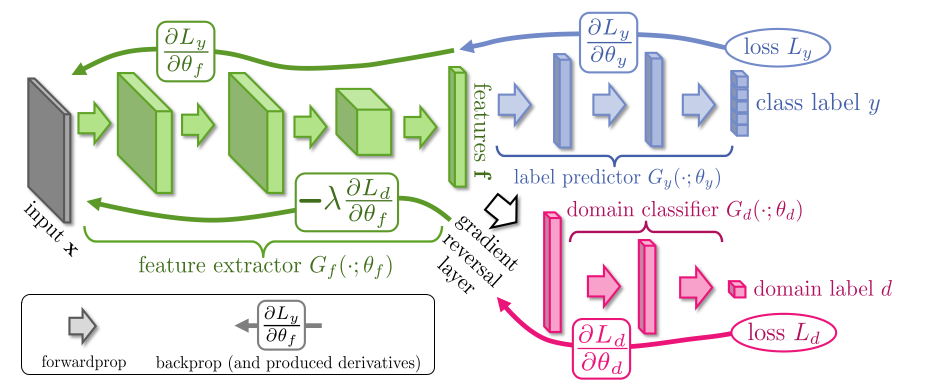
\includegraphics[width=0.8\textwidth]{Figures/From articles/uda_backpropagation.png}
    \caption{The proposed architecture includes a deep feature extractor (shown in green), a deep label predictor (shown in blue) and a domain classifier (shown in red). The domain classifier is connected to the feature extractor via a gradient reversal layer, which multiplies the incoming gradient by a negative constant during backpropagation-based training. The gradient reversal layer ensures that the feature distributions over the two domains become as similar as possible (i.e., indistinguishable by the domain classifier), resulting in domain-invariant features.}
    \label{fig: uda_back}
\end{figure}

The authors introduce an architecture that predicts both the label $y \in Y$ and the domain label $d \in \{0, 1\}$ for each input $\textbf{x}$. The architecture consists of three parts: feature extractor $\bold{f} = G_f(\textbf{x}, \theta_f)$, where $\theta_f$ is a vector that represents the parameters of all its layers; label predictor $G_y$ that maps the features obtained after feature extractor to the label $y$, with $\theta_y$ representing its parameters; domain classifier $G_d$ maps the same feature vector $\bold{f}$ to the domain label $d$, with $\theta_d$ representing its parameters. The purpose to minimize the label prediction loss for the source domain and simultaneously make the features $\textbf{f}$ invariant to the domain. To achieve this, the authors optimize the parameters $\theta_f$ of the feature mapping to maximize the loss of the domain classifier, however the parameters $\theta_d$ are optimized to minimize the loss of the domain classifier. The authors consider the loss

\begin{equation}
\begin{split}
E(\theta_f, \theta_y, \theta_d) & = \sum_{\substack{i=1..N \\ d_i = 0}} L_y(G_y(G_f(\textbf{x}_i; \theta_f); \theta_y), y_i) - \lambda \sum_{i = 1..N} L_d(G_d(G_f(\textbf{x}_i; \theta_f); \theta_d), y_i) \\ & = \sum_{\substack{i=0..N \\ d_i = 0}} L_y^i(\theta_f, \theta_y) - \lambda \sum_{i=1..N} L_d^i(\theta_f, \theta_d)
\end{split}
\end{equation} 

 where $L_y$ and $L_d$ are label prediction and domain classification losses, respectively. (index $i$ means the i-th example). It is considered the parameters $\hat{\theta}_f, \hat{\theta}_y, \hat{\theta}_d$ to gain a saddle point

\begin{equation}
\begin{split}
(\hat{\theta}_f , \hat{\theta}_y ) = \arg \min_{\theta_f, \theta_y} E(\theta_f, \theta_y, \hat{\theta}_d)
\\
\hat{\theta}_d = \arg \max_{\theta_d} E(\hat{\theta}_f, \hat{\theta}_y, \theta_d)
\end{split}
\end{equation}

During learning, the trade-off between the two objectives that shape the features is controlled by the parameter $\lambda$. The following stochastic updates can find a saddle point

\begin{equation}
\begin{split}
\theta_f & \leftarrow \theta_f - \mu \left( \dfrac{\partial L_y^i}{\partial \theta_f} - \lambda \dfrac{\partial L_d^i}{\partial \theta_f} \right) \\ 
\theta_y & \leftarrow \theta_y - \mu \dfrac{\partial L_y^i}{\partial \theta_y} \\ 
\theta_d & \leftarrow \theta_d - \mu \dfrac{\partial L_d^i}{\partial \theta_d} 
\end{split}
\end{equation} 

where $\mu$ is a learning rate. These updates are similar to SGD but with a $-\lambda$ factor in the first update to prevent dissimilar features across domains. Therefore, the authors introduce a GRL that acts as an identity transform during forward propagation but multiplies the gradient by $-\lambda$ during backpropagation.

\subsubsection{Second article}
Next, we continue with the article \textit{"Learning Semantic Representations for Unsupervised Domain Adaptation"} written by Xie, Shaoan, et al. \cite{xie2018learning} The main purpose of the article is to propose a new method for unsupervised domain adaptation that utilizes semantic information to learn domain-invariant representations. The authors propose a domain adaptation algorithm which is based on the idea of using an adversarial learning to learn a feature representation that is invariant to domain shifts. 

\begin{figure}[H]
    \centering
    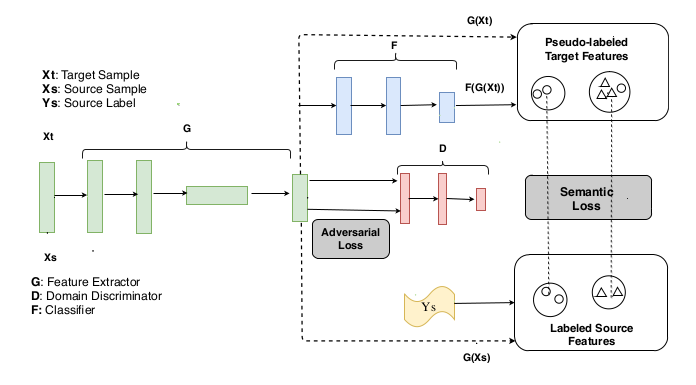
\includegraphics[width=0.7\textwidth]{Figures/From articles/sem_rep.png}
    \caption{The authors use standard source classification loss with the domain adversarial loss to align distribution for two domains. It is showed that the performance of the domain adaptation method improved significantly on several benchmark datasets by aligning the centroids. Global centroids $C_S^k$ and $C_T^k$ is maintained for each class at feature level.}
    \label{fig: sem_rep}
\end{figure}

 The authors train a feature extractor and then use it to map the input data to a high-dimensional feature space, and a domain classifier that predicts the domain label of the input data (see Figure \ref{fig: sem_rep}). The feature extractor \textbf{G} is trained to confuse the domain classifier \textbf{D}, while the domain classifier is trained to correctly predict the domain label. In this way, the feature extractor is encouraged to learn features that are invariant to domain shifts, while still being discriminative for the task.\\

 
 First, the authors denote the cross entropy loss for the source domain as $L_C(X_S, Y_S)$. Then, the discrepancy between source domain and target domain is supposed to be 

 $$
 L_{DC}(X_S, X_T) = d(X_S, X_T) = \mathbb{E}_{x \sim D_S} [\log(1 - D \circ G(x))] + \mathbb{E}_{x \sim D_T} [\log(D \circ G(x))] 
 $$
Moreover, the authors introduce one more loss, which targets the semantic representation. Centroid alignment is used for this purpose. By computing the centroid for each class, both correct and incorrect pseudo-labeled samples are utilized together: 

$$
L_{SM}(X_S, Y_S, X_T) = \sum_{k=1}^K \Phi(C_S^k, C_T^k)
$$
where $C_S^k, C_T^k$ are centroids for each class and $\Phi(x, x') = \| x - x' \|^2$. This approach aims to cancel out the negative effects caused by inaccurate pseudo labels with accurate ones. Thus, the authors get the following total loss

 $$
 L(X_S, Y_S, X_T) = L_C(X_S, Y_S) + \lambda L_{DC}(X_S, X_T) + \gamma L_{SM}(X_S, Y_S, X_T)
 $$
 where $\lambda$ and $\gamma$ are responsible for the balance between the classification
loss, domain confusion loss and semantic loss. In the article, algorithm of \textbf{moving average centroid alignment} is presented that allows to align the centroids in same class
but different domains to achieve semantic transfer for UDA.

\subsection{Fixbi for UDA}

The purpose of the article "Fixbi: Bridging domain spaces for unsupervised domain adaptation" written by Jaemin Na, Heechul Jung et al. \cite{na2021fixbi} is to propose a  fixed ratio-based mixup method to address the problem of large domain discrepancies. The authors mix up images and then fed them into neural networks to achieve greater reliability in learning from corrupted labels. It is proposed to use two predetermined mixup ratios $\lambda_sd$ and $\lambda_td$ for the source and target domain respectively. 
Denote input samples and their labels for source and target domain as $(x_i^s, y_i^s)$ and $(x_i^t, \hat{y}_i^t)$, the authors define mixup configurations in the following way:

\begin{equation}
\begin{split}
 \tilde{x}^{st}_i &= \lambda x_i^s + (1 - \lambda)x_i^t\\
 \tilde{y}^{st}_i &= \lambda y_i^s + (1 - \lambda)\hat{y}_i^t,
\end{split}
\end{equation} 

where $\lambda \in \{\lambda_{sd}, \lambda_{td} \}$ and $\lambda_{sd} + \lambda_{td} = 1$, $\hat{y}_i^t$ is the pseudo-labels for the target samples. By leveraging the fixed ratio-based mixup, it is constructed two neural networks with different perspectives: the "source-dominant model" (SDM) and the "target-dominant model" (TDM) (see Figure \ref{fig: fixbi}).

\begin{figure}[H]
    \centering
    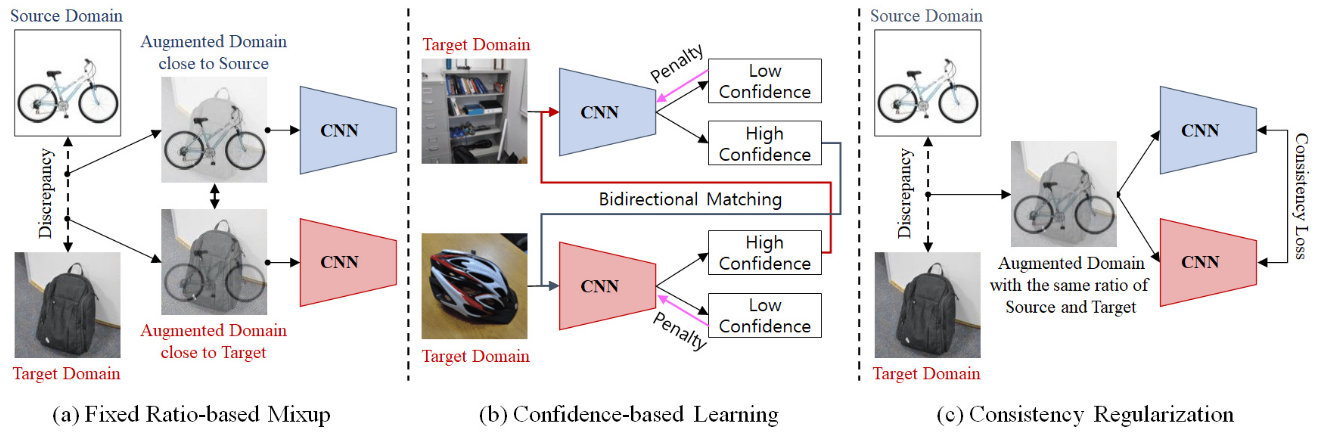
\includegraphics[width=\textwidth]{Figures/From articles/fixbi.png}
    \caption{All parts of FixBi training model: (a) fixed ratio-based mixup, (b)
confidence-based learning and (c) consistency regularization.}
    \label{fig: fixbi}
\end{figure}

The SDM provides robust supervision for the source domain but relatively weak supervision for the target domain, while the TDM has strong supervision for the target domain but weaker supervision for the source domain. Thus, denoting $p(y| \tilde{x}^{st}_i)$ as a predicted class distribution, it is defined fixed ratio-based mixup function 

\begin{equation}
\label{eq:fixbi1}
L_{fm} = \dfrac{1}{B} \sum_{i = 1}^B \hat{y}^{st}_i \log (p(y|\tilde{x}^{st}_i)),
\end{equation}

where $\hat{y}^{st}_i = \arg \max p(y|\tilde{x}^{st}_i)$ and $B$ is the size of a mini-batch. In order to have connections between source and target domains, it is suggested to use a confidence-based learning approach whereby one model educates the other using positive pseudo-labels, or penalties itself using negative pseudo-labels. Positive pseudo-labels means labels which predictions are above a specific threshold, then the authors use them in training the second model by utilizing a conventional cross-entropy loss. Thus, denote p and q as distributions of two models, the authors get the following loss function

\begin{equation}
L_{bim} = \dfrac{1}{B}\sum_{i=1}^B \mathds{1}(\max (p(y|x_i^t) > \tau)\hat{y}_i^t \log (q(y|x_i^t)),
\end{equation}

where $\hat{y}_i^t = \arg \max p(y|x_i^t)$. In contrast, a negative pseudo-label refers to the top-1 label predicted by the network with a confidence below the threshold $\tau$. The function of self-penalization is defined as follows:

\begin{equation}
L_{sp} = \dfrac{1}{B}\sum_{i=1}^B \mathds{1}(\max (p(y|x_i^t) < \tau)\hat{y}_i^t \log (1 - p(y|x_i^t))
\end{equation}
Furthermore, the threshold is changed adaptively during training. In addition, it is introduced the following expression: 

\begin{equation}
\label{eq:fixbi4}
L_{cr} = \dfrac{1}{B} \sum_{i=1}^B \| p(y|\tilde{x}^{st}_i) - q(y|\tilde{x}^{st}_i)\|^2_2
\end{equation}
that represents consistency regularization to guarantee a stable convergence during the training of both models.

\subsection{Spherical Space DA with Pseudo-label Loss}

Now we are going to the next article \textit{"Spherical Space Domain Adaptation with Robust Pseudo-label Loss"} written by  Xiang Gu, Jian Sun, and Zongben Xu. \cite{gu2020spherical} The authors propose a spherical space representation of data, which allows them to get more effective feature extraction and better adaptation across domains. One approach associated with increasing performance with differences in data distribution between source and target domain is to use pseudo-labels. However, the use of pseudo-labels can be problematic in the presence of noisy or incorrect labels. To tackle this problem, the authors map the data to a high-dimensional sphere and introduce a new loss function, called the robust pseudo-label loss, which is designed to address the problem of noisy or incorrect labels in the target domain. 

\begin{figure}[H]
    \centering
    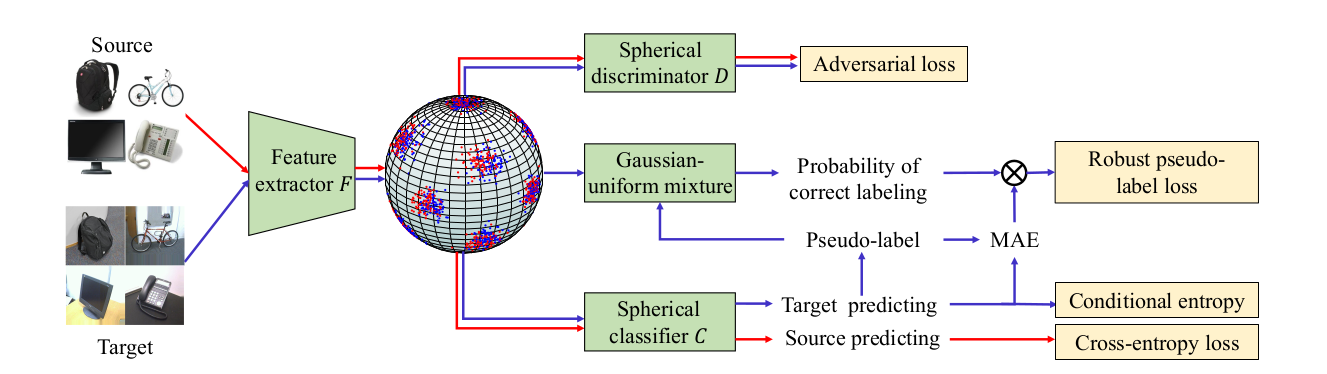
\includegraphics[width=\textwidth]{Figures/From articles/RSDA_scheme.png}
    \caption{Robust Spherical Domain Adaptation (RSDA) method proposed by the authors consists of a feature extractor F, which is a deep convolutional network, used to extract features that are then embedded onto a sphere, a spherical classifier and a discriminator that predict class labels and domain labels, respectively. Target pseudo-labels and features passing through the Gaussian-uniform mixture model are used to estimate the posterior probability of correct labeling.}
    \label{fig: RSDA_scheme}
\end{figure}

In the Figure \ref{fig: RSDA_scheme} we can see spherical domain adaptation method. Domain invariant features are learned by adversarial training, entirely in the spherical feature space.  The feature extractor F is utilized to normalize the features to map onto a sphere. The classifier C and discriminator D are defined in the spherical feature space, consisting of spherical perceptron layers and a spherical logistic regression layer (see Figure \ref{fig: sphere_layers}). 

\begin{figure}[H]
    \centering
    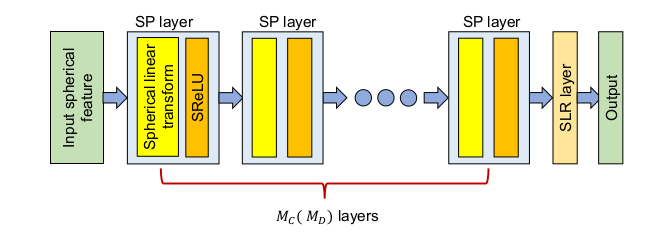
\includegraphics[width=0.7\textwidth]{Figures/From articles/sphere_layers.png}
    \caption{Spherical neural network structure}
    \label{fig: sphere_layers}
\end{figure}

Although the use of a spherical element reduces feature dimension by one, it simplifies the domain adaptation process by eliminating differences in norms. The authors define spherical adversarial training loss as follows:

\begin{equation}
    L = L_{bas}(F, C, D) + L_{rob}(F, C, \phi) + \gamma L_{ent}(F)
\end{equation}

This lost consists of three parts: basic loss, robust pseudo-label loss and conditional entropy loss. Let's start with the first one. To align features, the authors utilize basic loss which is defined as an adversarial domain adaptation loss:
\begin{equation}
L_{bas}(F, C, D) = L_{src}(F, C) + \lambda L_{adv}(F, D) + \lambda' L_{sm}(F),
\end{equation}
where $L_{src}$ is a cross-entropy loss for the source domain, $L_{adv}$ is an adversarial training loss and $L_{sm}$ is a semantic loss. The second one is conditional entropy loss which is used to keep the learned features away from the classification boundary:
\begin{equation}
L_{ent}(F) = \dfrac{1}{N_t} \sum_{j=1}^{N_t} H(C(F(x_j^t))),
\end{equation}
where $H(\cdot)$ denotes the entropy of a distribution. Additionally, the authors propose robust pseudo-label loss to increase robustness of the model. Denote $\tilde{y}_j^t = \arg \max_k [C(F(x_i^s))]_k$ as a pseudo-lebel of $x_j^t$ where $[\cdot]_k$ means the $k$-th element. To be ensured in precision of pseudo-labels, it is assumed to use new random variable $z_j \in \{0, 1\}$ for each pair $(x_j^t, \tilde{y}_j^t)$ that specify the correctness of the data (1 is correct, 0 is not). Let the probability of correct labeling be $P_\phi (z_j = 1| x_j^t, \tilde{y}_j^t)$ and $\phi$ to its parameters, then robust loss is defined as follows:

\begin{equation}
L_{rob}(F, C, \phi) = \dfrac{1}{N_0}\sum_{j=1}^{N_t} w_\phi(x_j^t) \mathcal{J}(C(F(x_j^t)), \tilde{y}_j^t),
\end{equation}
where $N_0 = \sum_{j=1}^{N_t} w_\phi(x_j^t)$ and $\mathcal{J}(\cdot, \cdot)$ is mean absolute error (MAE). The function $w_\phi (x_j^t)$ is defined using the posterior probability of correct labeling 

\begin{equation}
w_\phi(x_j^t) = \left\{\begin{split}
\gamma_j,& \;\; \text{if } \gamma_j \geq 0.5,\\
0,& \;\; \text{otherwise},
\end{split}\right.
\end{equation}
where $\gamma_j = P_\phi(z_j = 1| x_j^t, \tilde{y}_j^t)$. By utilizing a Gaussian-uniform mixture model in spherical space based on pseudo-labels, the authors model the probability $P_\phi(z_j = 1| x_j^t, \tilde{y}_j^t)$ as a function of the feature distance between the data and the center of the corresponding class. Thus, samples from target domain with a probability of correct labeling below 0.5 can be discarded. For further details of computing posterior probability, please refer to the article \cite{gu2020spherical}.  

\subsection{DA with Invariant Representation Learning}
 Next, we move on to the article \textit{"Domain Adaptation with Invariant Representation Learning: What Transformations to Learn?"} written by Stojanov, Petar, et al. \cite{stojanov2021domain} The researchers focus on the conditional shift scenario, where the data-generating process is utilized to (\textbf{i}) explain why two distinct encoding functions are required to infer the latent representation, (\textbf{ii}) improve an implementation of these functions, and (\textbf{iii}) impose meaningful structure on the latent representation $Z$ to increase prediction accuracy in the target domain.

\begin{figure}[H]
    \centering
    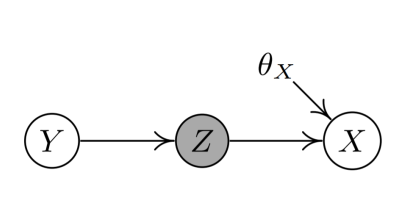
\includegraphics[width=0.5\textwidth]{Figures/From articles/DA_transforms.png}
    \caption{Data-generating process under conditional shift}
    \label{fig: DA_transf}
\end{figure}

Let's consider the data-generating process shown in the Figure \ref{fig: DA_transf} to understand what information is required for learning. The label $Y$ is generated first from its prior distribution $P(Y)$. Then, the invariant representation $Z$ is generated from $Y$ through $P(Z|Y)$, and $X$ is generated from $P(X|Z; \theta_X)$, where $\theta_X$ represents the changing parameters of $P(X|Y)$ across domains. We can consider $Z$ as a latent representation of our data. The variable $\theta_X$ may correspond to environment-specific changes that are irrelevant for predicting the class $Y$. Generally speaking, $Z$ is conditionally dependent on $\theta_X$ given $X$, although they may be marginally independent. Therefore, to recover $Z$ given $X$, the information of $\theta_X$ should also be considered in the transformation (see detailed in the article to understand clearly how authors measure the influence of $\theta_X$). The authors made two key observation associated with the data-generating process. Firstly, the encoder function $\phi$ requires $\theta_X$ as an input in addition to X. Secondly, assuming that $\theta_X$ has minimal influence on the relationship between $X$ and $Z$, allowing us to use a single encoder $\phi(X, \theta_X)$ instead of two separate encoders. A decoder function $\widetilde{\phi}$ that restricts the influence of $\theta_X$, acting as a regularizer on the encoder $\phi$, in order to retain important semantic information.

\begin{figure}[H]
    \centering
    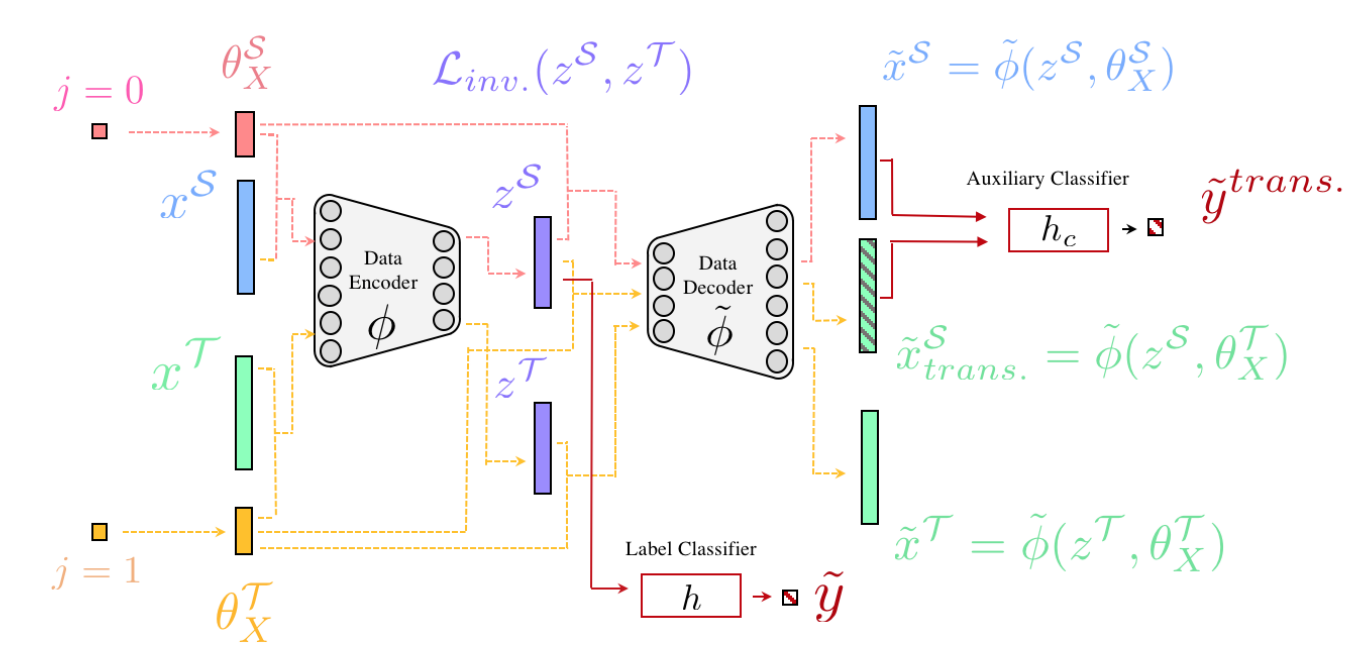
\includegraphics[width=0.85\textwidth]{Figures/From articles/DA_cnn.png}
    \caption{Autoencoder framework used in this article}
    \label{fig: DA_cnn}
\end{figure}

Thus, the authors proposed a domain-adaptation network, which is shown in the Figure \ref{fig: DA_cnn}, where $\theta_X \in \{\theta_X^S, \theta_X^T\}$ parameters for source and target domains respectively. 

\subsection{Domain Adaptation for Segmentation with CBST}

The main purpose of the paper \textit{"Domain Adaptation for Semantic Segmentation via Class-Balanced Self-Training"} written by Zou, Yang, et al. \cite{zou2018unsupervised} propose a new UDA framework for semantic segmentation based on iterative self-training procedure. A novel technique, referred to as Class-Balanced Self-Training (CBST), has been suggested by the authors, which aims to adapt the segmentation model from the source domain to the target domain by leveraging unlabeled target data. In the Figure \ref{fig: sem_seg}, the authors present a structure and the results of their deep self-training framework using two datasets: GTA 5 \cite{richter2016playing} and Cityscapes \cite{cordts2016cityscapes}.

\begin{figure}[H]
    \centering
    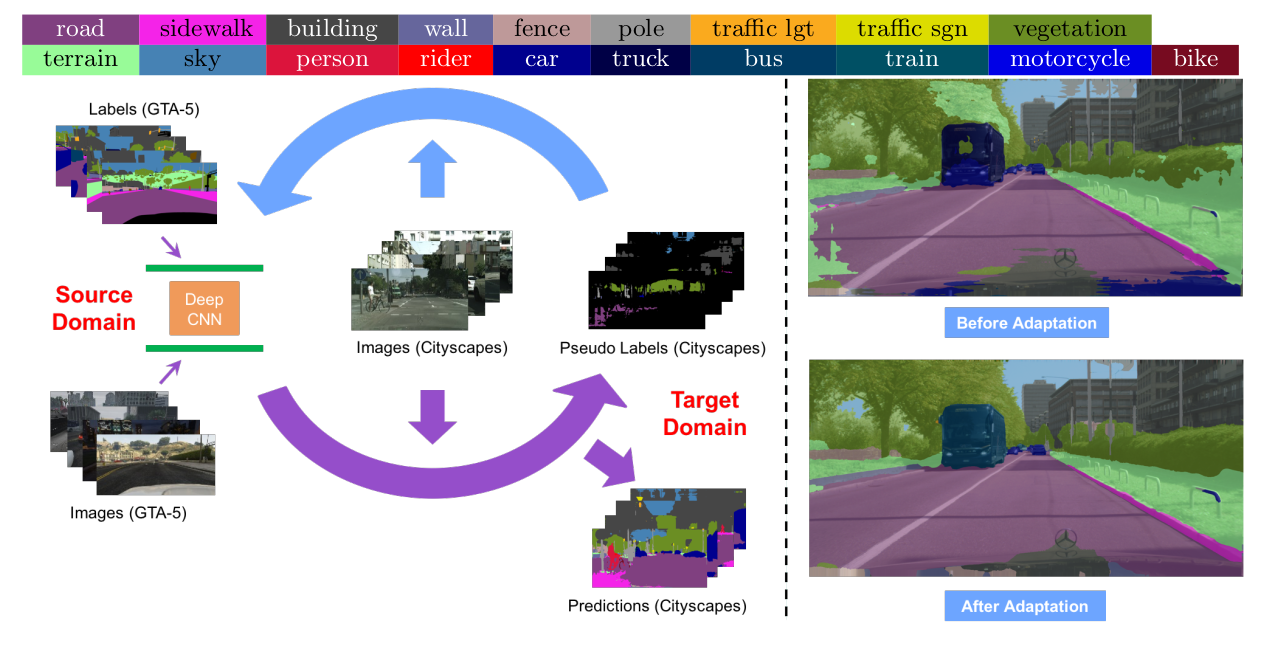
\includegraphics[width=0.8\textwidth]{Figures/From articles/semantic_segmentation.png}
    \caption{ On the left side, the self-training framework for UDA is presented. On the right side, obtained results before and after adaptation for the Cityscapes dataset.}
    \label{fig: sem_seg}
\end{figure}

The CBST approach is based on two main components: a class-balancing strategy and a self-training algorithm. The class-balancing strategy aims to address the problem of class imbalance between the source and target domains, which can negatively impact the performance of the segmentation model. The authors change the loss function using parameters that determine the proportion of selected pseudo-labels due to balance the class distribution during the self-training process. Furthermore, when the images in the source and target domains are similar, spatial prior knowledge can be effectively utilized to adapt models. For this purpose, the authors count the class frequencies in the source domain using Gaussian kernel. The experimental results show that the CBST approach outperforms several state-of-the-art unsupervised domain adaptation methods for semantic segmentation. 



